\documentclass[titlepage]{article}
\usepackage[T2A]{fontenc}
\usepackage[utf8]{inputenc}
\usepackage[russian]{babel}

\usepackage{amsmath}
\usepackage{graphicx}
\graphicspath{ {../images/} }

\begin{document}

\begin{titlepage}

\begin{center}
	Министерство науки и высшего образования Российской Федерации\\
	Федеральное государственное автономное образовательное учреждение\\
	высшего образования\\
	\textbf{«Уральский федеральный университет\\
	имени первого президента России Б. Н. Ельцина»}
\end{center}

\vspace*{9em}{\centering\Huge
	Итоговая рассчётная работа по статистике\par}
\vspace{9em}

\begin{flushright}
	Дубовиков Н.Ю. \\ РИ-200003 \\ Преподователь Поторочина К.С.
\end{flushright}

\mbox{}
\vfill
\begin{center}
	Екатеринбург\\
	2021
\end{center}
\clearpage
\end{titlepage}

\tableofcontents
\newpage

\section{Введение}
\subsection{Предмет исследования}

Предметом данного иссследования является зависимость числа умышленных убийств (убийств первой степени
в законодательстве Соединённых Штатов) от количества владельцев оружия в разных городах США.

\subsection{Описание случайных величин}

Величины берутся в единицах на сто тысяч человек. Исходные данные были загружены с сайта ФБР. Данные актуальны на 2019 год.
\par
Количество умышленных убийств --- количество известных ФБР правонарушений, связанных с умышленным причинением смерти, произошедших
в 2019 году на территории определённого города.
\par
Количество владельцев оружия --- общее число граждан США, живущих на территории определённого города, получивших от ФБР разрешение
на покупку оружия. Определяется в основном строгостью законов в штате или городе, потому может сильно отличаться на разных
территориях страны. \par
Случайная выборка из ста значений исследуемых случайных величин представлена в таблице в приложении~\ref{sec:appendix} (названия городов
указаны как в оригинале --- на английском).

\subsection{Актуальность исследования}

Исследование позволяет установить, помогает ли ограничение оборота оружия снизить количество преступлений, связанных с насилием,
в частности убийств. Этим подтверждается её актуальность.

\subsection{Цель исследования}

Цель работы --- установить, есть ли зависимость между количеством умышленных убийств и количеством владельцев оружия на душу населения.

\section{Часть первая. Исследование одномерной выборки}

При исследовании одномерной выборки будем использовать величину X --- количество умышленных убийств на $100 000$ человек.
Объём выборки $N = 100$.

\subsection{Вариационный ряд}

Найдем из выборки минимальное и максимальное значение. $X_{min} = 0, X_{max} = 636$. Далее во формуле Стерджиса находим оптимальное количество интервалов:
\begin{equation*}
k = 1 + 3.332lg(N) \approx 7.35 \approx 7
\end{equation*}

Чтобы включить больше значений в крайние интервалы, возьмём $k = 6$ (при $k = 7$ в два крайних интервала попадёт $3 - 4$ значения).
Из размаха значений выборки и количества интервалов найдём длину одного интервала:
\begin{equation*}
h = \frac{X_{max} - X_{min}}{k} = 106
\end{equation*}

Теперь составим вариационный ряд:
\begin{table}[!ht]
    \centering
    \begin{tabular}{|l|l|l|l|l|l|l|}
    \hline
        Интервал & $[0; 106]$ & $(106; 212]$ & $(212; 318]$ & $(318; 424]$ & $(424; 530]$ & $(530; 636]$ \\ \hline
        $n_i$ & 31 & 25 & 14 & 10 & 8 & 6 \\ \hline
    \end{tabular}
\end{table}

\subsection{Полигон и гистограмма частот}
Построим полигон и гистограмму относительных частот. Для этого вычислим относительные частоты по формуле:
\begin{equation*}
w_i = \frac{n_i}{N}
\end{equation*}
Также найдём середины всех интервалов и занесём все значения в таблицу:
\begin{table}[!ht]
    \centering
    \begin{tabular}{|l|l|l|l|l|l|l|}
    \hline
        Интервал & $[0; 106]$ & $(106; 212]$ & $(212; 318]$ & $(318; 424]$ & $(424; 530]$ & $(530; 636]$ \\ \hline
        $n_i$ & 31 & 25 & 14 & 10 & 8 & 6 \\ \hline
        $x_i$ & 53 & 159 & 265 & 371 & 477 & 583 \\ \hline
        $w_i$ & 0.329 & 0.265 & 0.148 & 0.106 & 0.085 & 0.063 \\ \hline
    \end{tabular}
\end{table}

По этой таблице сделаем полигон и гистограмму частот:

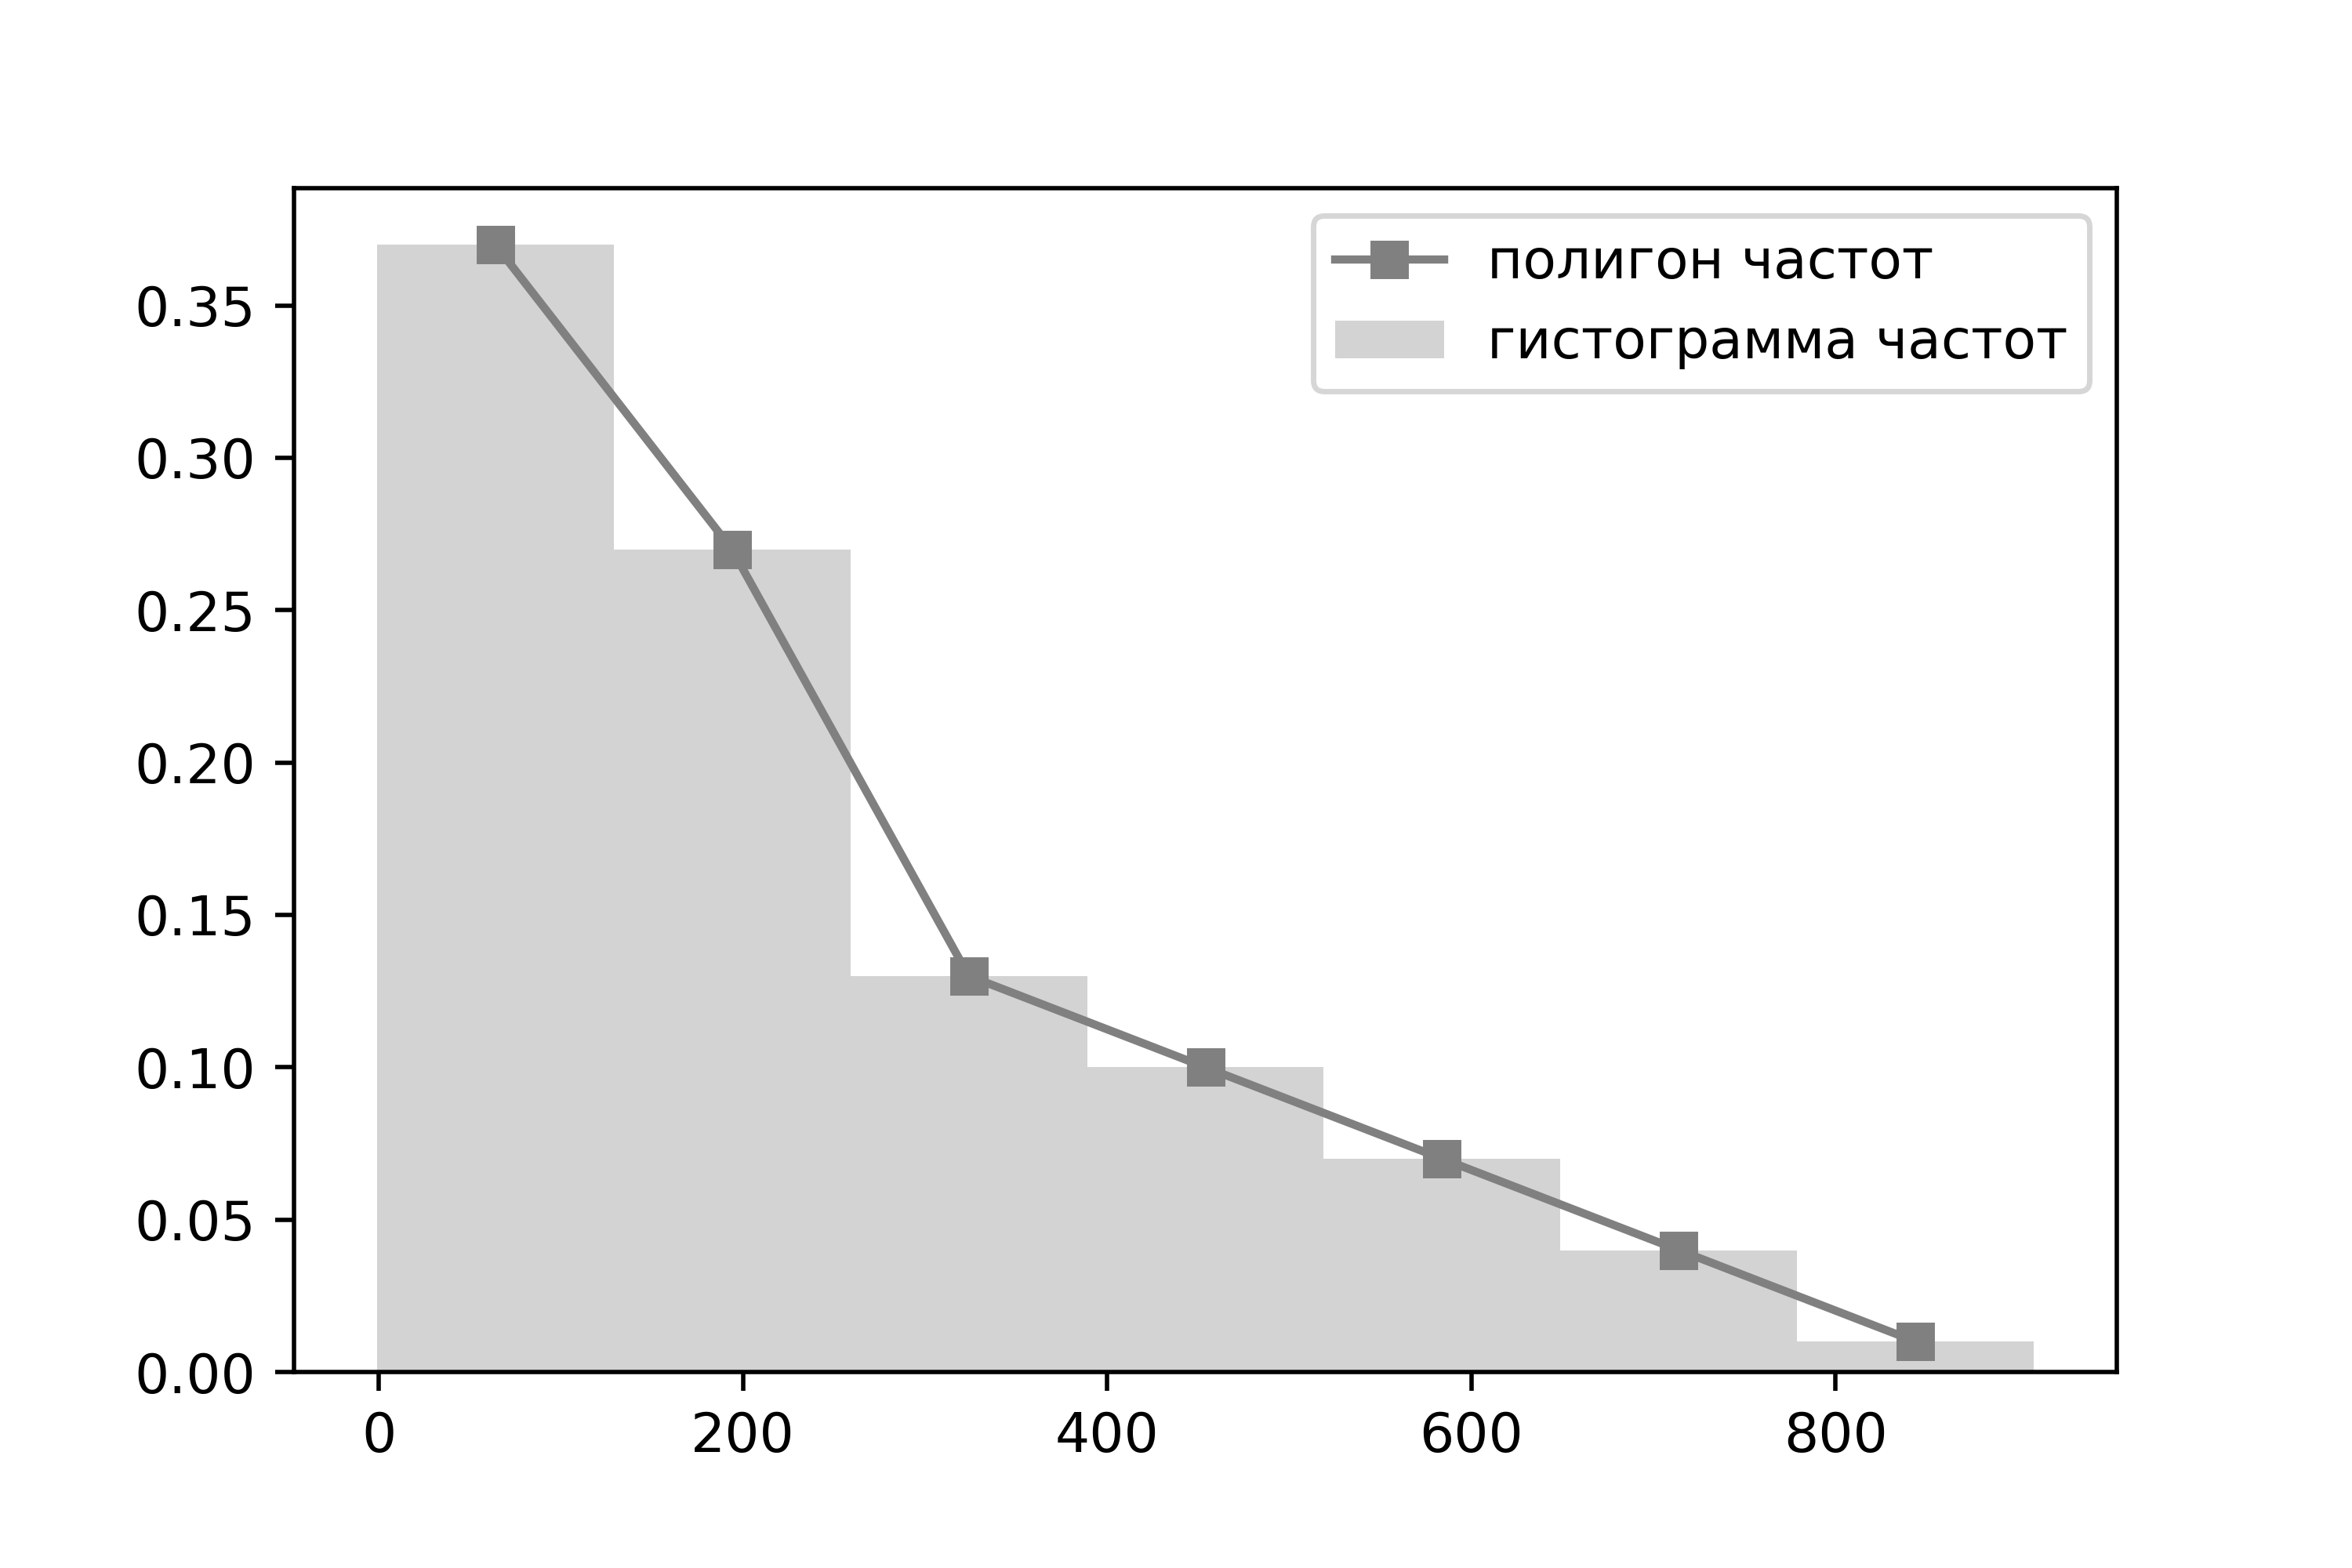
\includegraphics[scale=0.6]{fig01}

\subsection{Эмпирическая функция распределения}
Для того, чтобы найти эмпирическую функцию распределения, необходимы накопительные частоты, они вычисляются по формуле:
\begin{equation*}
W_i = \sum_{k = 0}^{i} w_k
\end{equation*}
То есть это сумма всех предыдущих относительных частот. Так же внесём всё в таблицу:

\begin{table}[!ht]
    \centering
    \begin{tabular}{|l|l|l|l|l|l|l|}
    \hline
        Интервал & $[0; 106]$ & $(106; 212]$ & $(212; 318]$ & $(318; 424]$ & $(424; 530]$ & $(530; 636]$ \\ \hline
        $n_i$ & 31 & 25 & 14 & 10 & 8 & 6 \\ \hline
        $w_i$ & 0.329 & 0.265 & 0.148 & 0.106 & 0.085 & 0.063 \\ \hline
        $W_i$ & 0.33 & 0.59 & 0.74 & 0.85 & 0.94 & 1 \\ \hline
    \end{tabular}
\end{table}

По получившимся значениям построим график:

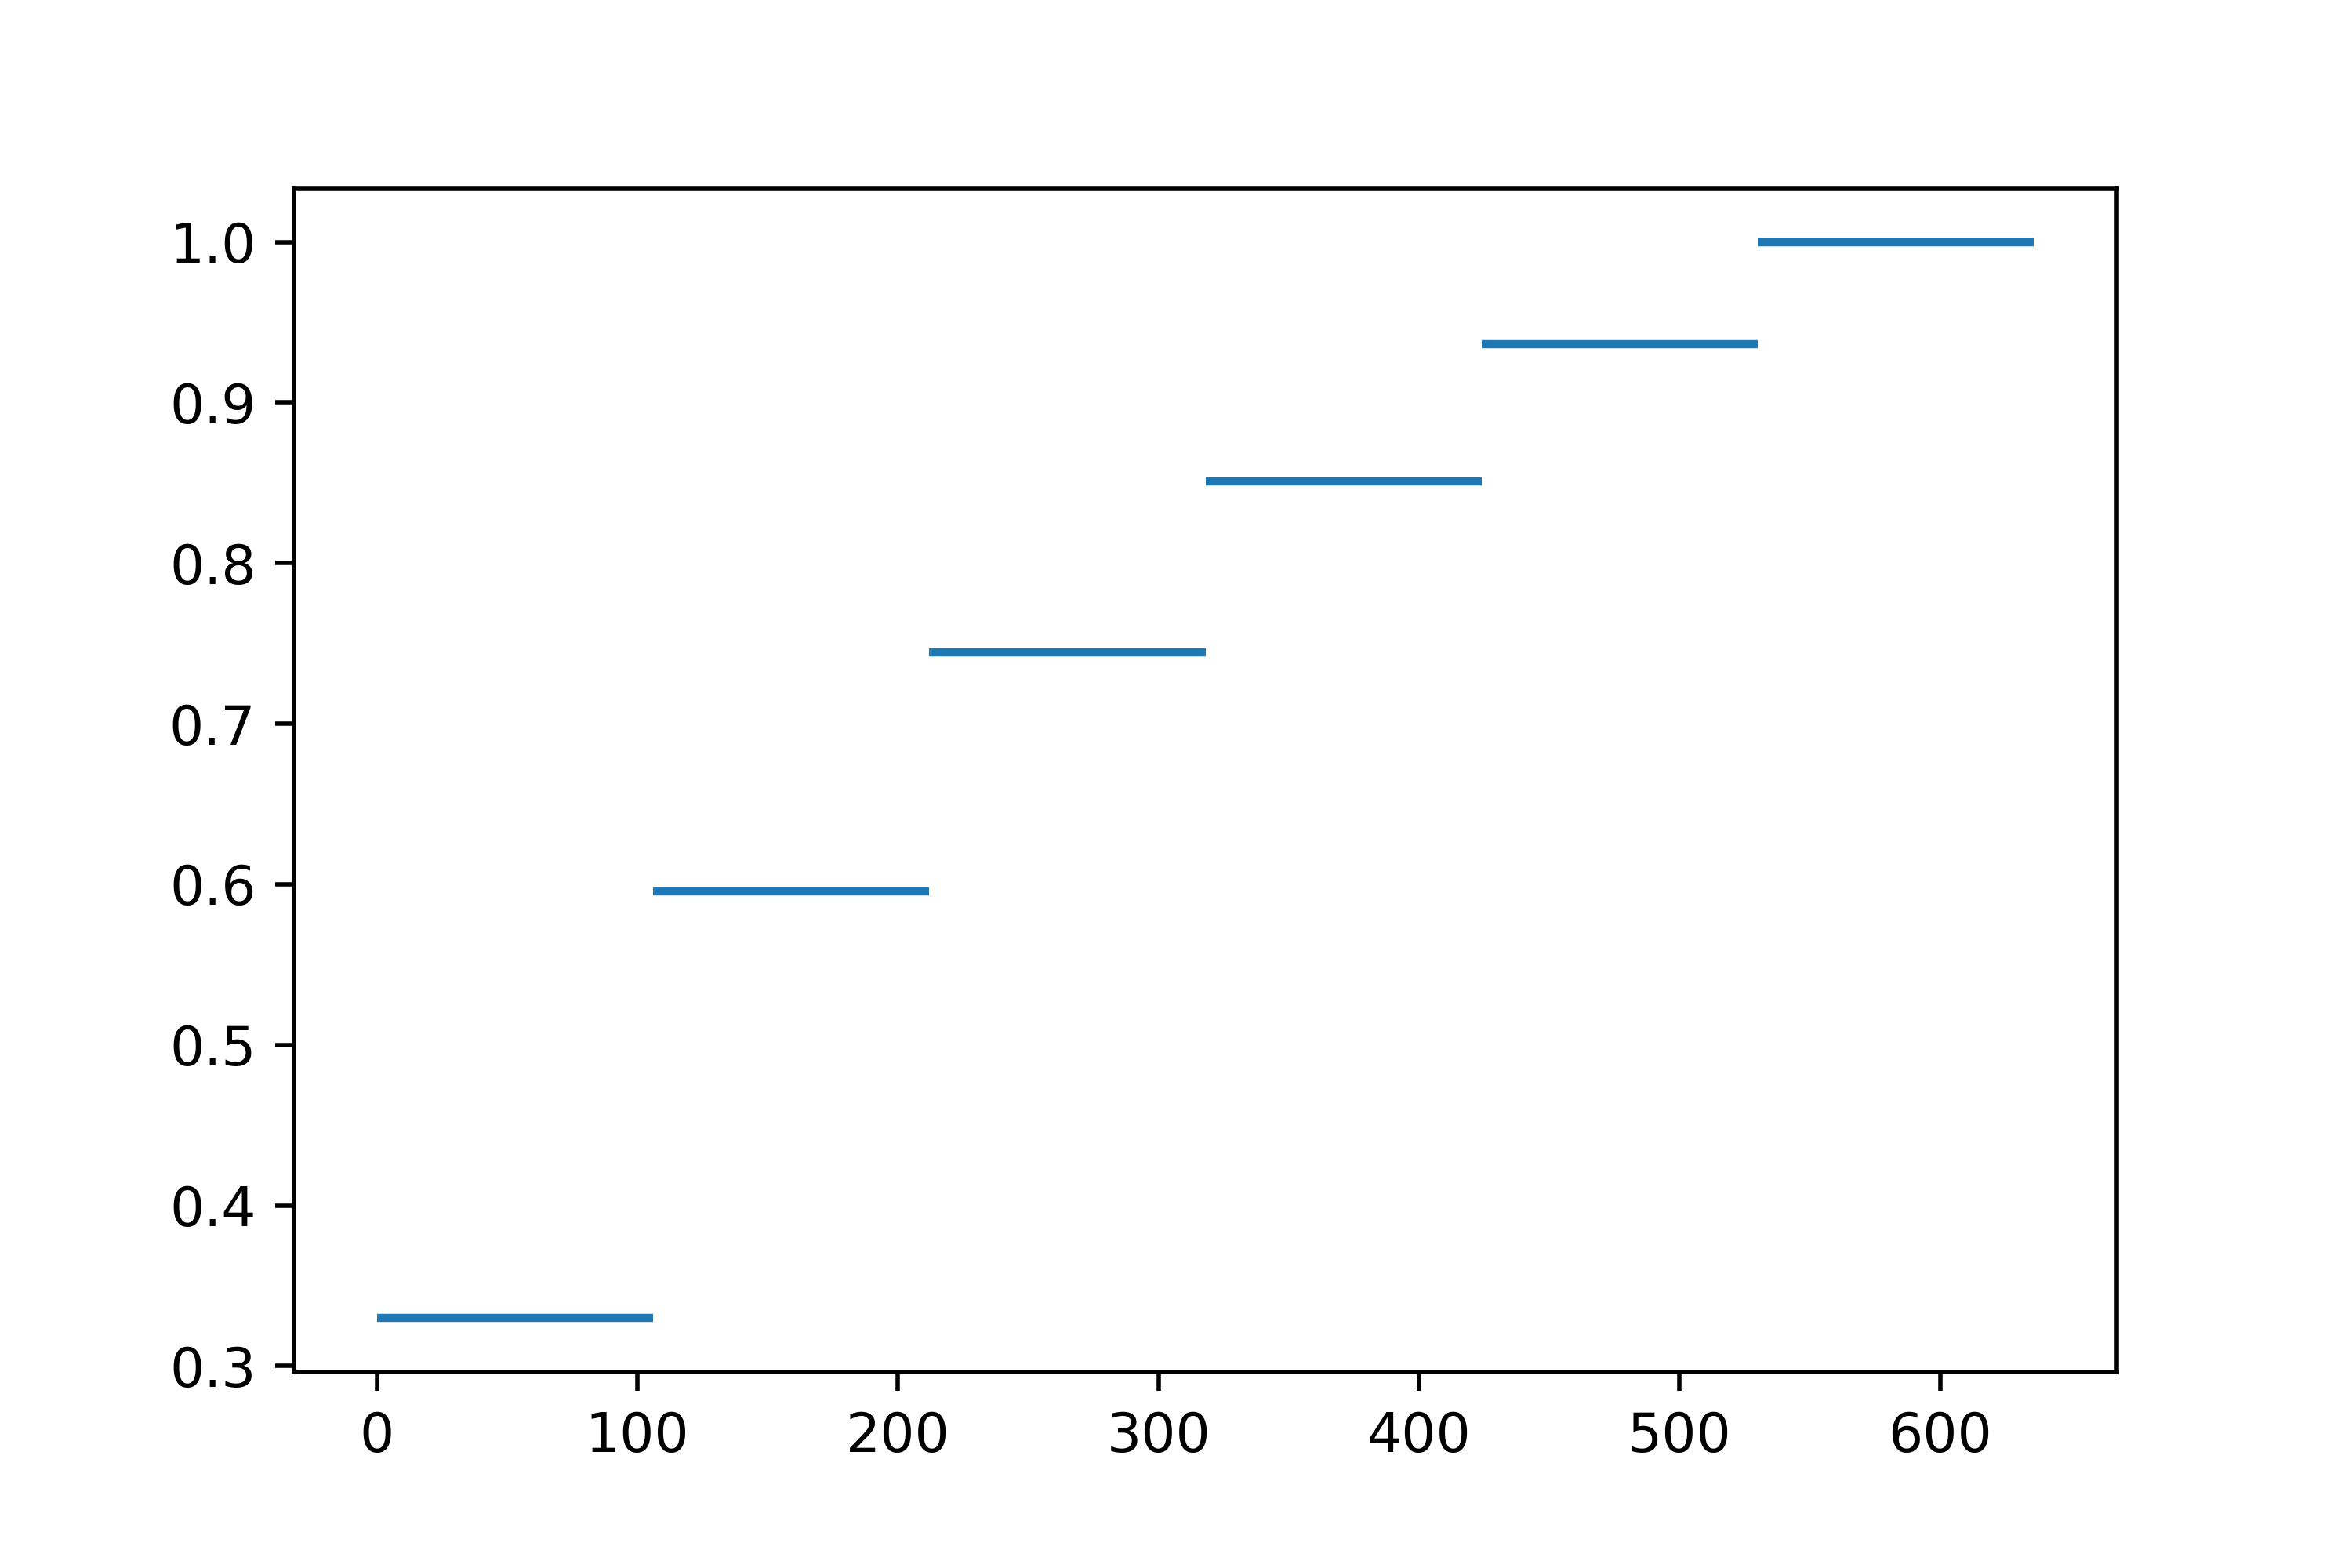
\includegraphics[scale=0.6]{fig02}

\subsection{Числовые характеристики}
Рассчитаем выборочную среднюю, дисперсию, среднее квадратичное отклонение, асимметрию и эксцесс.

\begin{itemize}

\item
Выборочная средняя (значения $x_i$ и $n_i$ возьмём из таблицы выше):
\begin{equation*}
\overline{X}_B = \frac{1}{N} \sum_{i = 1}^N x_i n_i \approx 216.51
\end{equation*}

\item
Выборочная дисперсия:
\begin{equation*}
D_B = \frac{1}{N} \sum_{i = 1}^N (x_i - \overline{X}_B)^2 n_i \approx 26934.1
\end{equation*}

\item
Исправленная дисперсия:
\begin{equation*}
S^2 = \frac{N \cdot D_B}{N - 1} \approx 27223.7
\end{equation*}

\item
Среднее квадратическое отклонение:
\begin{equation*}
\sigma = \sqrt{D_B} \approx 164.116
\end{equation*}

\item
Исправленное среднее квадратическое отклонение:
\begin{equation*}
S = \sqrt{S^2} \approx 164.996
\end{equation*}

\item
Ассиметрия --- мера смещения графика влево-вправо:
\begin{equation*}
A = \frac{1}{N S^3} \sum_{i = 1}^N (x_i - \overline{X}_B)^3 n_i \approx 0.793
\end{equation*}

\item
Эксцесс --- мера высоты графика:
\begin{equation*}
e_x = \frac{1}{N S^4} \sum_{i = 1}^N (x_i - \overline{X}_B)^4 n_i \approx -0.512
\end{equation*}
\end{itemize}

\subsection{Доверительный интервал}
Определим доверительный интервал для оценки математического ожидания при надежности $\gamma = 0.95$.
Доверительный интервал – интервал, который покрывает неизвестный параметр с заданной надёжностью.
\begin{equation*}
\overline{X}_B - \delta < a < \overline{X}_B + \delta
\end{equation*}
Где $\delta = \frac{t_{\gamma} S}{\sqrt N}$. Из уравнения $\Phi (t_{\gamma}) = \gamma$ вычислим, что $t_{\gamma} \approx 1.96$. Тогда $\delta \approx 33.355$.

Следовательно интервал $183.155 < a < 249.866$ покрывается с надёжностью  $\gamma = 0.95$.

\subsection{Уровень значимости по критерию Пирсона}
Рассчитаем уровень значимости $\alpha$, при котором распределение для выборки согласуется с нормальным законом по критерию согласия Пирсона ($\chi^2$).
Выдвинем гипотезы:

\begin{itemize}
	\item $H_0$ --- распределение является нормальным.
	\item $H_1$ --- распределение нормальным не является.
\end{itemize}

Функция нормального распределения $F (x) = \frac{1}{2} + \Phi(\frac{x - a}{\sigma})$.
\begin{equation*}
P(X_i < x < X_{i+1}) = F(X_{i+1}) - F(X_i) = \Phi \left( \frac{x_{i+1} - \overline{X}_B}{S} \right) - \Phi \left(\frac{x_i - \overline{X}_B}{S} \right)
\end{equation*}

\clearpage
Занесём все значения, необходимые для рассчётов, в таблицу:
\begin{table}[!ht]
    \centering
    \begin{tabular}{|l|l|l|l|l|l|l|l|l|}
    \hline
		$X_i$ & $X_{i+1}$ & $\frac{x_i - \overline{X}_B}{S}$ & $\frac{x_{i+1} - \overline{X}_B}{S}$ & $\Phi \left( \frac{x_{i+1} - \overline{X}_B}{S} \right)$ & $\Phi \left(\frac{x_i - \overline{X}_B}{S} \right)$ & $P$ & $nP$ & $\frac{(n - nP)^2}{nP}$ \\ \hline
		0 & 106 & 31 & -1.312 & -0.669 & -0.405 & -0.248 & 0.156 & 14.736 \\ \hline
		106 & 212 & 25 & -0.669 & -0.027 & -0.248 & -0.010 & 0.237 & 22.333 \\ \hline
		212 & 318 & 14 & -0.027 & 0.615  & -0.010 &  0.230 & 0.241 & 22.716 \\ \hline
		318 & 424 & 10 & 0.615  & 1.257  &  0.230 &  0.395 & 0.164 & 15.506 \\ \hline
		424 & 530 &  8 & 1.257  & 1.899  &  0.395 &  0.471 & 0.075 &  7.102 \\ \hline
		530 & 636 &  6 & 1.899  & 2.542  &  0.471 &  0.494 & 0.023 &  2.182 \\ \hline
    \end{tabular}
\end{table}

Откуда $\chi^2 = \sum \frac{(n_i - n_i P)^2}{n_i P} \approx 30.358$. В результате уровень значимости $\alpha \approx 1.16 \cdot 10^{-6}$. На вычисленном уровне значимости принимается нулевая гипотеза.

\subsection{Выводы}
Гипотеза о нормальном распределении была отклонена. Из эксцесса и коэффициента ассиметрии следует, что распределение отклонено вправо и вниз относительно нормального.

\section{Часть вторая. Исследование двумерной выборки}
\subsection{Первые начальные моменты}
\begin{equation*}
v_{10} = \overline{X}_B = \sum_{i=1}^N x_i n_{xi} \approx 216.51
\end{equation*}
\begin{equation*}
v_{01} = \overline{Y}_B = \sum_{i=1}^N y_i n_{yi} \approx 41231.91
\end{equation*}

\subsection{Вторые центральные моменты}
\begin{equation*}
\mu_{20} = \frac{1}{N} \sum_{i = 1}^N (x_i - \overline{X}_B)^2 n_{xi} \approx 26934.1
\end{equation*}
\begin{equation*}
\mu_{02} = \frac{1}{N} \sum_{i = 1}^N (y_i - \overline{Y}_B)^2 n_{yi} \approx 106076853.77
\end{equation*}

Коэффициент ковариации:
\begin{equation*}
K_{xy} = \overline{XY} - X_B \cdot Y_B
\end{equation*}

\clearpage
Составим корреляционную таблицу:
\begin{table}[!ht]
    \centering
    \begin{tabular}{|l|l|l|l|l|l|l|}
    \hline
        ~ & [14700;23300] & (23300;31900] & (31900;40500] & (40500;49100] & (49100;57700] & (57700;66300] \\ \hline
        [0;106] & 0 & 5 & 4 & 16 & 6 & 0 \\ \hline
        (106;212] & 1 & 2 & 4 & 13 & 5 & 0 \\ \hline
        (212;318] & 0 & 4 & 2 & 6 & 2 & 0 \\ \hline
        (318;424] & 2 & 2 & 0 & 3 & 1 & 2 \\ \hline
        (424;530] & 0 & 4 & 0 & 2 & 2 & 0 \\ \hline
        (530;636] & 2 & 0 & 2 & 0 & 2 & 0 \\ \hline
    \end{tabular}
\end{table}

И таблицу, в которой на пересечении $i$-й строки и $j$-го столбца находится значение $n_{ij} \cdot x_i \cdot y_j$:

\begin{table}[!ht]
    \centering
    \begin{tabular}{|l|l|l|l|l|l|l|}
    \hline
        ~ & 19000 & 27600 & 36200 & 44800 & 53400 & 62000 \\ \hline
        53.0 & 0 & 5035000 & 4028000 & 16112000 & 6042000 & 0 \\ \hline
        159.0 & 4388400 & 8776800 & 17553600 & 57049200 & 21942000 & 0 \\ \hline
        265.0 & 0 & 38372000 & 19186000 & 57558000 & 19186000 & 0 \\ \hline
        371.0 & 33241600 & 33241600 & 0 & 49862400 & 16620800 & 33241600 \\ \hline
        477.0 & 0 & 101887200 & 0 & 50943600 & 50943600 & 0 \\ \hline
        583.0 & 72292000 & 0 & 72292000 & 0 & 72292000 & 0 \\ \hline
    \end{tabular}
\end{table}

Используя эту таблицу можно посчитать $\overline{XY}$ (сложить всё и поделить на объём выборки).

\begin{equation*}
\overline{XY} = \frac{1}{N} \sum \sum x_i y_j n_{ij} \approx 9171142.55
\end{equation*}

Тогда $K_{xy} \approx 243994.34$. Откуда коэффициент корреляции:
\begin{equation*}
r_{xy} = \frac{K_{xy} }{ \sqrt{\mu_{20} \cdot \mu_{02} } } \approx 0.144
\end{equation*}

По таблице Чеддока, связь между величинами слабая. Проверим гипотезу $H_0$ о том, что $r_{xy} = 0$, а так же альтернативную гипотезу $H_1$: $r_{xy} \ne 0$.
\begin{equation*}
T = \frac{r_{xy} \sqrt{n - 2} }{\sqrt{1 - r^2_{xy} } } \approx 1.399
\end{equation*}

При $N - 2 = 92$ степенях свободы коэффициент Стьюдента при уровне значимости 0.05  равен 1.98.
$|T| < t_K$, поэтому гипотезу $H_0$ принимаем, то есть X и Y не коррелируют.
\clearpage

\subsection{Эмпирическая линия и прямая регрессии}

Регрессия Y по X: $y = r_{xy} \frac{\mu_{02} }{\mu_{20} } (x - v_{10}) - v_{01}$.
Для вычисления составим таблицу произведений $y_i$ на число появлений из корреляционной таблицы $n_{ij}$:
\begin{table}[!ht]
    \centering
    \begin{tabular}{|l|l|l|l|l|l|l|}
    \hline
        Y | X               & (0;106] & (106;212] & (212;318] & (318;424] & (424;530] & (530;636] \\ \hline
        (14700;23300] &      0 &  27600 &      0 &  89600 &      0 & 124000 \\ \hline
        (23300;31900] &  95000 &  55200 & 144800 &  89600 & 213600 &      0 \\ \hline
        (31900;40500] &  76000 & 110400 &  72400 &      0 &      0 & 124000 \\ \hline
        (40500;49100] & 304000 & 358800 & 217200 & 134400 & 106800 &      0 \\ \hline
        (49100;57700] & 114000 & 138000 &  72400 &  44800 & 106800 & 124000 \\ \hline
        (57700;66300] &      0 &      0 &      0 &  89600 &      0 &      0 \\ \hline
		Сумма & 117800.0 & 40588.235 & 42233.333 & 11200.0 & 23733.333 & 186000.0 \\ \hline
    \end{tabular}
\end{table}

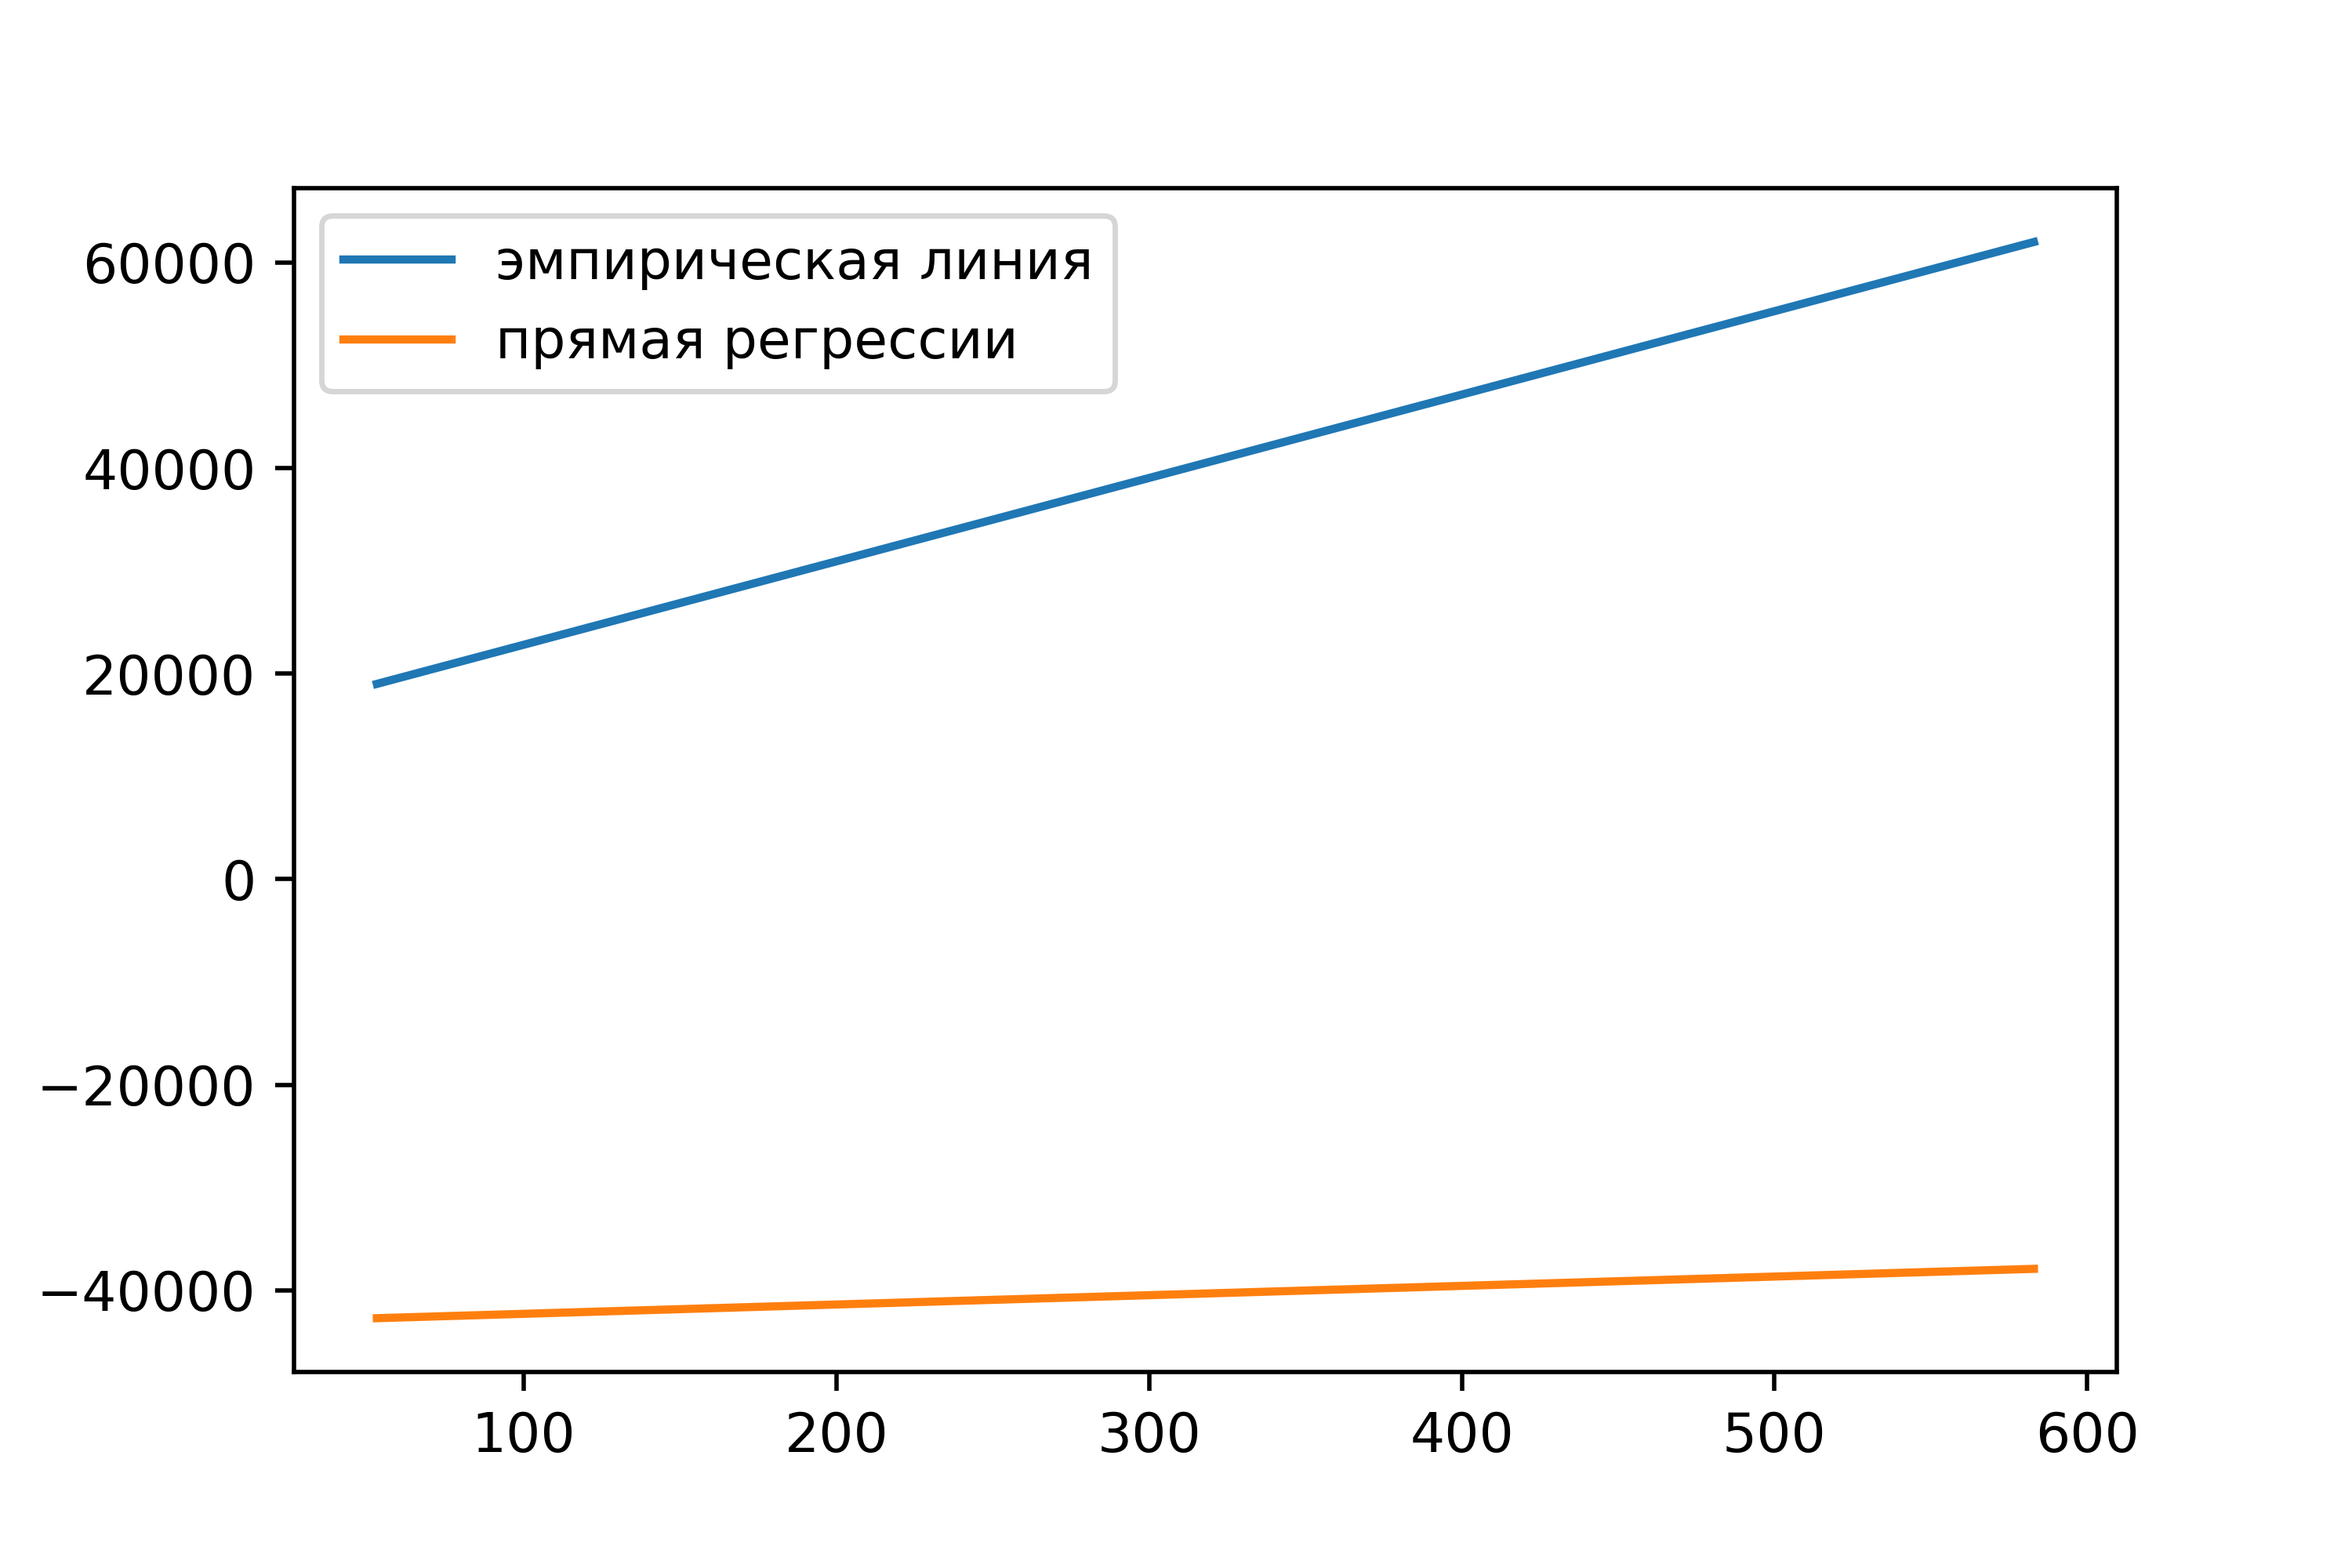
\includegraphics[scale=0.6]{fig03}

\clearpage
\appendix
\section{Выборка из собранных данных}
\label{sec:appendix}
\begin{table}[!ht]
    \centering
    \begin{tabular}{|l|l|l|}
    \hline
        Город & Количество убийств & Количество владельцев оружия \\ \hline
        Buckeye & 137 & 46300 \\ \hline
        Nevada & 255 & 48800 \\ \hline
        Dilley & 223 & 45700 \\ \hline
        GrossePointe & 117 & 40200 \\ \hline
        NewHaven & 297 & 44800 \\ \hline
        Harrisonville & 277 & 48800 \\ \hline
        Boston, & 607 & 14700 \\ \hline
        OakGrove & 207 & 48800 \\ \hline
        Tomahawk & 96 & 45300 \\ \hline
        Winchester & 481 & 51600 \\ \hline
        Hulbert & 171 & 54700 \\ \hline
        Emerson & 0 & 45200 \\ \hline
        Winneconne & 80 & 45300 \\ \hline
        VillaPark & 157 & 27800 \\ \hline
        BradentonBeach & 155 & 35300 \\ \hline
        Beatrice & 180 & 45200 \\ \hline
        Northglenn & 457 & 45100 \\ \hline
        Hutchinson & 378 & 48900 \\ \hline
        WarminsterTownship & 84 & 40700 \\ \hline
        Lyndhurst & 104 & 40000 \\ \hline
        Bath & 48 & 46800 \\ \hline
        Redmond & 102 & 42100 \\ \hline
        RobinsonTownship & 124 & 40700 \\ \hline
        Streetsboro & 121 & 40000 \\ \hline
        Chickasha & 433 & 54700 \\ \hline
        Murphy & 43 & 45700 \\ \hline
        Melbourne & 692 & 35300 \\ \hline
        Killeen & 384 & 45700 \\ \hline
        Maumee & 103 & 40000 \\ \hline
        Hanford & 449 & 28300 \\ \hline
        Pembroke & 92 & 44600 \\ \hline
        Elwood & 133 & 27800 \\ \hline
        Ashburnham & 126 & 14700 \\ \hline
        Athol & 402 & 14700 \\ \hline
        HedwigVillage & 224 & 45700 \\ \hline
        Elkton & 103 & 44600 \\ \hline
        Clarkdale & 68 & 46300 \\ \hline
        Auburn & 146 & 46800 \\ \hline
        Bokchito & 581 & 54700 \\ \hline
        Corning & 372 & 28300 \\ \hline
    \end{tabular}
\end{table}
\begin{table}[!ht]
    \centering
    \begin{tabular}{|l|l|l|}
    \hline
        Город & Количество убийств & Количество владельцев оружия \\ \hline
        Madison & 84 & 45200 \\ \hline
        Hastings & 246 & 40200 \\ \hline
        RanchoCordova & 297 & 28300 \\ \hline
        Viola & 0 & 27800 \\ \hline
        Jonesville & 272 & 40200 \\ \hline
        Ackerman & 139 & 55800 \\ \hline
        Mazon & 103 & 27800 \\ \hline
        SouthHaven & 555 & 40200 \\ \hline
        Fishers & 53 & 44800 \\ \hline
        Orion & 56 & 27800 \\ \hline
        Plymouth & 327 & 14700 \\ \hline
        Federalsburg & 528 & 30200 \\ \hline
        NewLondon & 294 & 23600 \\ \hline
        Niles & 774 & 40200 \\ \hline
        Rossville & 0 & 51600 \\ \hline
        LaVergne & 392 & 51600 \\ \hline
        Somerset & 0 & 40000 \\ \hline
        Emporia & 240 & 44600 \\ \hline
        Rosenberg & 380 & 45700 \\ \hline
        EagleVillage & 47 & 45300 \\ \hline
        Franklin & 165 & 51600 \\ \hline
        Ellensburg & 211 & 42100 \\ \hline
        Hemet & 398 & 28300 \\ \hline
        RomanForest & 148 & 45700 \\ \hline
        Perry & 245 & 54700 \\ \hline
        Refugio & 109 & 45700 \\ \hline
        Norfork & 0 & 57200 \\ \hline
        OliverSprings & 58 & 51600 \\ \hline
        Williamstown & 0 & 54600 \\ \hline
        Wynona & 0 & 54700 \\ \hline
        Dunwoody & 128 & 49200 \\ \hline
        Verona & 990 & 48800 \\ \hline
        Chicopee & 615 & 14700 \\ \hline
        GenevaTown & 40 & 45300 \\ \hline
        Avon & 63 & 42800 \\ \hline
        Auburn & 73 & 54600 \\ \hline
        Clinton & 160 & 54600 \\ \hline
        Mathis & 440 & 45700 \\ \hline
        Okmulgee & 615 & 54700 \\ \hline
        Newport & 806 & 50500 \\ \hline
        Halifax & 164 & 44600 \\ \hline
        Kirtland & 88 & 40000 \\ \hline
    \end{tabular}
\end{table}
\begin{table}[!ht]
    \centering
    \begin{tabular}{|l|l|l|}
    \hline
        Город & Количество убийств & Количество владельцев оружия \\ \hline
        Adrian & 689 & 40200 \\ \hline
        PalmSprings & 636 & 35300 \\ \hline
        FrontRoyal & 183 & 44600 \\ \hline
        MissouriCity & 141 & 45700 \\ \hline
        Visalia & 434 & 28300 \\ \hline
        PigeonForge & 736 & 51600 \\ \hline
        Beebe & 279 & 57200 \\ \hline
        Manhattan & 375 & 66300 \\ \hline
        Williamston & 176 & 40200 \\ \hline
        Berkeley & 503 & 28300 \\ \hline
        BerwynHeights & 214 & 30200 \\ \hline
        Muscatine & 197 & 43600 \\ \hline
        WilkinsTownship & 49 & 40700 \\ \hline
        LakeZurich & 40 & 27800 \\ \hline
        Merrillville & 144 & 44800 \\ \hline
        Buhl & 360 & 60100 \\ \hline
        PalosHeights & 40 & 27800 \\ \hline
        Martinez & 215 & 28300 \\ \hline
    \end{tabular}
\end{table}

\mbox{}
\vfill

\end{document}
